\section{Diseño experimental}

El diseño experimental se lo realizó usando el algoritmo J48, el cual es una implementación de \cite{hall2009weka}
desarrollado por Ross Quinlan. Éste a su vez es una extensión del algoritmo ID3, del mismo autor.

En los diseños experimentales se dividieron en dos dos partes, un 80\% de las instancias
se utilizaron para el entrenamiento del árbol, mientras que el 20\% restante se utilizó para
testearlo. La división se hizo de forma aleatoria, manteniendo la misma proporción de clases en cada
uno de los subconjuntos de datos.

Para la implementación de los experimentos se utilizó la biblioteca 'RWeka' \cite{rweka}, una implementación de los algoritmos de 
WEKA para lenguaje de programación R, el código fuente de la implementación puede ser consultada en el repositorio\footnote{
Repositorio tp1AA \url{https://github.com/poldrosky/tp1AA}}.

\subsection{Sobreajuste y poda}

Se conoce como sobreajuste u overfitting, al efecto que consiste en pegarse mucho a los 
datos de entrenamiento, dicho en otros términos, sobre-entrenar el árbol,
perjudicando la performance sobre el conjunto de validación. \cite{mitchell1997machine}
define el overfitting como: ``A hypothesis overfits the training examples if some other hypothesis that
fits training examples less well actually performs better over the entire distribution of instances.''

\textbf{Metodología utilizada:} Se ejecutaron corridas del algoritmo J48 variando la función de
poda. Para ello, se utilizó como parámetro el ConfidenceFactor (CF). Se iteró desde 2,5 \%
a 50 \%, con intervalos de 2,5 \%. A menor porcentaje de CF, el algoritmo incurre en un mayor nivel
de poda. 

\textbf{Resultados esperados:} En función de lo enunciado en la descripción precedente, se
espera que a medida que crezca el tamaño del árbol, medido en función de la cantidad de
nodos, crezca monótonamente la performance sobre el conjunto de entrenamiento, y
luego disminuya sobre el de validación. Asi mismo, por cómo opera el CF, el tamaño del
árbol debería aumentar a medida que crece su valor.

\textbf{Análisis de los resultados:} Los resultados obtenidos una vez realizado el experimento
se pueden resumir en las figuras presentadas a continuación:

La figura~\ref{fig:over}a se observa que a medida que se incrementa el valor del CF la
cantidad de nodos también crece, mostrando una clara relación positiva entre el CF y el
tamaño del árbol; en ese sentido cabe recordar que ``The default confidence value is set at
25\% and works reasonably well in most cases; possibly it should be altered to a lower
value, which causes more drastic pruning'' \cite{witten2005data}; es decir que un valor bajo del CF implica una
poda muy grande y por otro lado un valor muy alto señalaría que el árbol no sufriría poda
alguna. Es razonable entonces que en el gráfico una poda muy grande esté asociada a
una poca cantidad de nodos y por el contrario una poda pequeña se vincule a una
cantidad grande de nodos, debido a que se dejó crecer el árbol sin ninguna restricción; sin
embargo esta figura, tomada de manera aislada, no dice absolutamente nada acerca de la
performance de la técnica predictiva sobre el conjunto de entrenamiento y de validación.

La figura~\ref{fig:over}b es la que muestra la relación entre la performance y el CF. Es
importante recordar que un CF mayor significa un menor nivel de poda y, teniendo en
cuenta la relación puesta en evidencia en el gráfico anterior, un incremento del tamaño del
árbol. De este gráfico es importante destacar que a medida que el árbol es más grande la
performance sobre el conjunto de entrenamiento es mayor, en tanto que en el caso del conjunto
de validación, el rendimiento también crece hasta un cierto nivel, para luego disminuir y
finalmente estabilizarse manteniéndose casi constante. Todo lo mencionado hace
suponer que si se toman valores muy grande de CF se colapsaría en el fenómeno
conocido como overfitting, donde el árbol de decisión clasifica muy bien las instancias 
pertenecientes al conjunto de entrenamiento, sin embargo no llega a tener una predicción
adecuada sobre nuevas instancias no conocidas.


\textbf{Conclusión:} Los resultados obtenidos se alinean con los esperados. Para el conjunto de
datos utilizado en el experimento, el árbol crecerá a medida que los niveles de poda se
restrinjan mediante la elección del valor del CF. Este crecimiento del árbol influirá
positivamente sobre la performance en el conjunto de entrenamiento; sin embargo en el caso
de los datos de validación el crecimiento del árbol tendrá un efecto positivo sobre su
performance hasta un cierto punto, siendo perjudicial una vez superado ese límite. Por lo
que parece recomendable elegir un valor de CF entre 0.1 y 0.2, que maximizaría los
niveles de predicción sobre los datos no conocidos. Asimismo esto se traducirá en árboles
con lenguajes de hipótesis no tan expresivos, pero que explicarán mejor los hechos; los
cuales según Occam son las teorías preferibles en condiciones similares.
``Occam’s Razor shaves philosophical hairs off a theory''.


En la figura~\ref{fig:over}c se muestra la grafica de la curva ROC para el mejor árbol, el cual
tiene una precisión 0.714.


\begin{figure*}
  \centering
  \subfigure[Leaves vs CF]{\label{b1} 
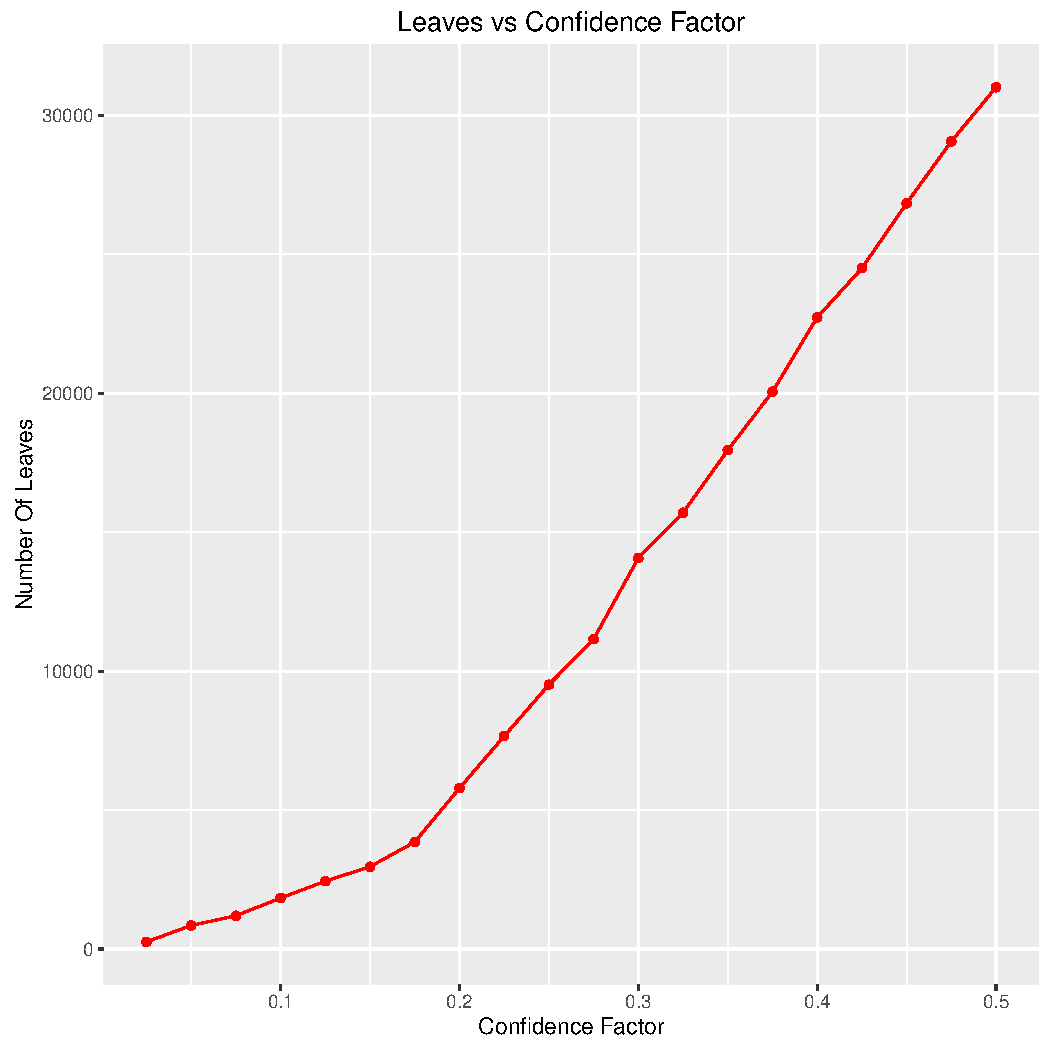
\includegraphics[width = 7cm]{3a.pdf}}
  \subfigure[Accuracy vs CF]{\label{b2}
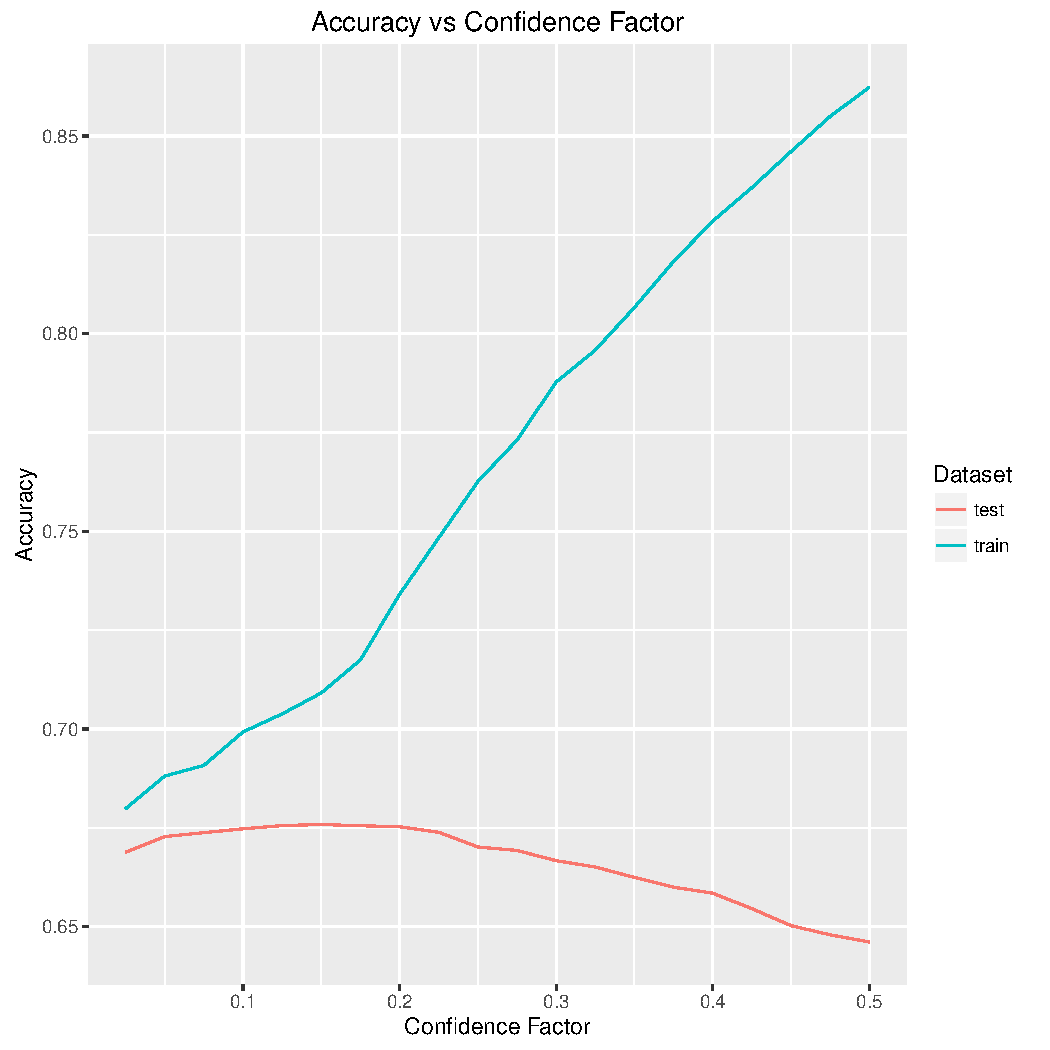
\includegraphics[width = 7cm]{3b.pdf}}
    \subfigure[ROC curve better tree]{\label{b3}
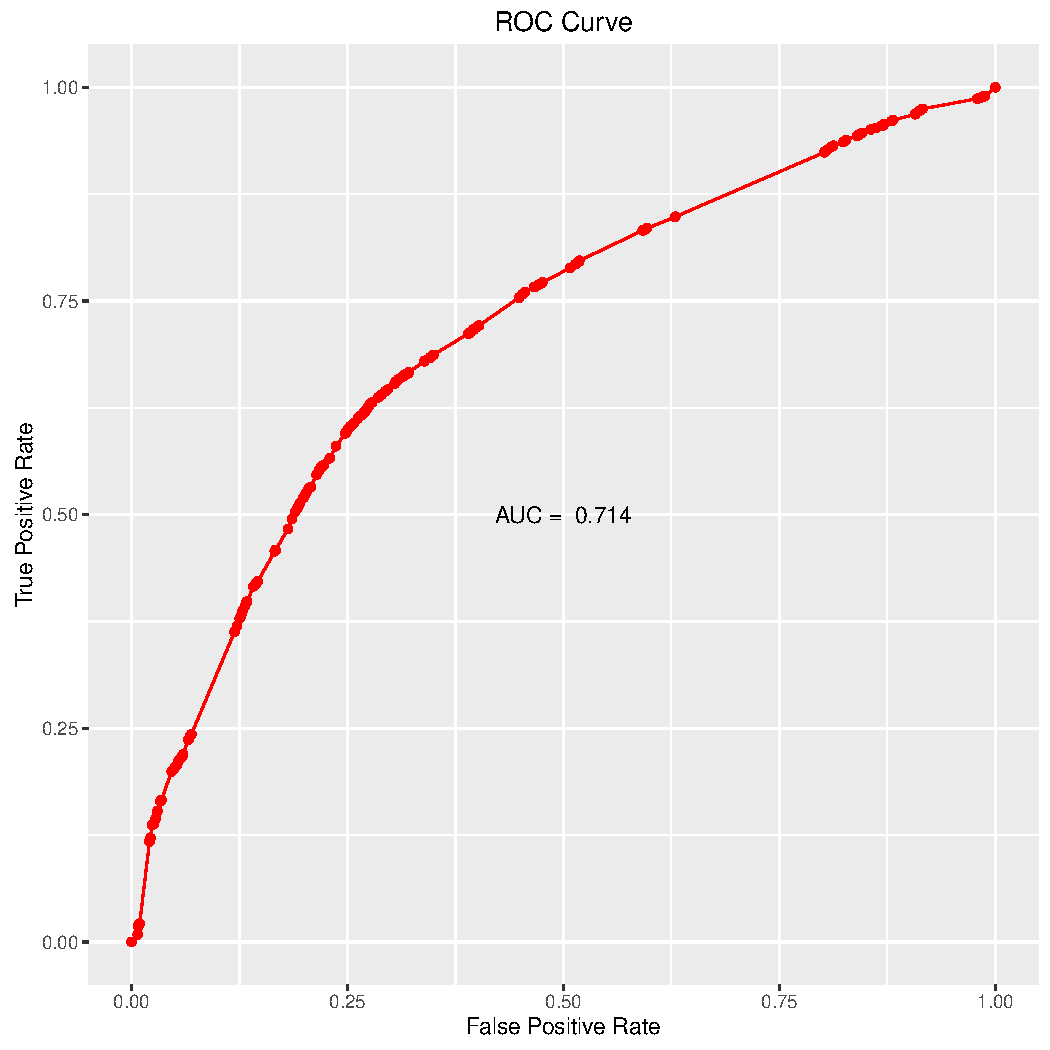
\includegraphics[width = 7cm]{3c.pdf}}
  \caption{overfitting and pruning}
  \label{fig:over}
\end{figure*}

